\documentclass{VUMIFInfKursinis}
\usepackage{algorithmicx}
\usepackage{algorithm}
\usepackage{algpseudocode}
\usepackage{amsfonts}
\usepackage{amsmath}
\usepackage{bm}
\usepackage{color}
\usepackage{graphicx}
% \usepackage{hyperref}  % Nuorodų aktyvavimas
\usepackage{url}
\usepackage{subcaption}	% You need this package for subfigures


% Titulinio aprašas
\university{Vilniaus universitetas}
\faculty{Matematikos ir informatikos fakultetas}
\institute{Informatikos institutas}  % Užkomentavus šią eilutę - institutas neįtraukiamas į titulinį
\department{Informatikos katedra}
\papertype{Kursinis darbas}
% Nenurodytas vienas arba keli iš būtinų atributų: kalba, raktiniai žodžiai, santrauka.
\title{Automatizuotas kriptovaliutų prekybos robotas}
\titleineng{Automated cryptocurrency trading bot}
\status{4 kurso 1 grupės studentas}
\author{Matas Kaminskas}
\supervisor{J. Asist., Dr. Igor Katin}
\date{Vilnius \\ \the\year}

% Nustatymai
% \setmainfont{Palemonas}   % Pakeisti teksto šriftą į Palemonas (turi būti įdiegtas sistemoje)
\bibliography{bibliografija} 

\begin{document}
\maketitle

\tableofcontents

% Įvade apibūdinamas darbo tikslas, temos aktualumas ir siekiami rezultatai. 
\sectionnonum{Įvadas}
% could be better, say something about novel nature of cryptocurrency
Pasaulis vis labiau modernėja, technologijos tampa vis išmanesnės ir našesnės, nei bet kada anksčiau. Šiais laikais turime kontraversiškai pagarsėjusią
kriptovaliutų rinką, kuri yra kaip skaidresnė atsvara standartinei akcijų biržai. Po 2007-2008 metų įvykusios finansų krizės,
visai neužilgo - \cite{nakamoto2008bitcoin} 2008 metais, atsirado pirmoji kriptovaliuta - Bitcoin. Tai yra decentralizuotą ir nepriklausoma elektroninę valiutą, paremta
blokų grandinės technologija. Dabartiniais apskaičiavimais šios rinkos bendra vertė viršija 800 milijardų JAV dolerių \cite{CoinMarketCap},
nors kiek daugiau nei prieš metus ši vertė buvo dvigubai didesnė - 1.6 trilijonų JAV dolerių, o tarp 2018 ir 2020 metų vertė daugmaž buvo stabili - apie 100 milijardų JAV dolerių.
Šie duomenys dar kartą pabrėžia kriptovaliutų rinkos nepastovumą, bei ženkliai padidėjusi susidomėjimą, populiarumą visuomenėje.    


Pagrindinis skirtumas tarp kriptovaliutų rinkos ir tradicines akcijų biržos yra jog mainai vyksta 24 valandas per parą. Akcijų biržoje yra nustatytos pagrindinės darbo valandos,
jos dažniausiai yra tokios pat kaip vietos darbo valandos ir pagrindiniai mainai vyksta šiomis valandomis, todėl stebėti tendencijas ir realizuoti strategijas yra įmanomas darbas asmeniui.
Kai rinka yra prieinama visa parą dirbant be sustojimo yra nepraktiška, bei neįmanoma stebėti ir atlikti prasmingus mainus rinkoje. Atsiranda puiki terpė automatizuoti šį 
procesą - įdarbinti automatizuotą prekybos robotą, kuris gebėtų analizuoti rinkos duomenis ir prognozuoti tolimesnė rinkos eigą.


Šio darbo tikslas yra sukurti automatizuota kriptovaliutų prekybos robotą naudojant standartinius laiko eilutės autoregresinius modelius. 
Darbe tiriama, kokį autoregresinį modelį galima taikyti: AR, ARMA, ARIMA, ARFIMA, SARIMA ar kt., tiksliausiai nuspėti kriptovaliutos
kainas ateityje. Pagal gautus rezultatus ir tikslumą galima spręsti, koks modelis yra tinkamiausias robotui naudoti.


Tikslui įgyvendinti keliami uždaviniai:
% bullet points
\begin{itemize}
  \item Mokslinės literatūros analizė, % kriptovaliutų, laiko eilučių ir autoregresinių modelių tema;
  \item Atlikti autoregresinių modelių analizę, %Autoregresinių modelių analizė ir jų paruošimas prognozuoti kainą.
  \item Sukurti automatizuotą robotą galintį pritaikyti autoregresinius modelius,
        % \item Ekspermentiškai ištirti autoregresinius modelius juos taikant robotui;
  \item Ištirti gautus rezultatus atlikus modelių taikymą, % ištirti
  \item Apibendrinti tyrimo metu gautus rezultatus ir apibrėžti išvadas.
\end{itemize}


%Pagrindinėje tiriamojoje dalyje aptariama ir pagrindžiama tyrimo metodika; ARFIMA AR MODELIAI IR T.t.
%pagal atitinkamas darbo dalis, nuosekliai, panaudojant lyginamosios analizės,
%klasifikacijos, sisteminimo metodus bei apibendrinimus, dėstoma sukaupta ir
%išanalizuota medžiaga.
\section{Pagrindinė tiriamoji dalis}
Pagrindinė ir pirmoji kriptovaliuta visoje rinkoje - Bitcoin. Stebint kriptovaliutų rinka matoma, jog nuo šios valiutos kainos koreliuoja visos kitos kriptovaliutų kainos.
Kyla bitcoin kainą - kyla kitų valiutų kainą, krenta bitcoin kainą - krenta kitų valiutų kainą. Retais atvejais kriptovaliuta sparčiau keičia kainą dėl pažangaus vystymosi ar dėl
% SOL auga labai? XRP freeze del teismo? ADA kyla nes pazangi, nors btc stabilus? ir kiti E.g. nezinu ar reikia čia šitą plėstis
esančių vidinių problemų. Dauguma kriptovaliutų yra riboto kiekio, tad jeigu prekybos robotas per laiko tarpą uždirba maža procentą, jų kainą gali keleriopai išaugti
tikrų valiutų atžvilgiu. Vienas iš uždavinių suprasti kaip veikia kriptovaliutų rinka, jog būtų galima automatizuoti šį robotą. Kriptovaliutų rinkoje, kaip ir
akcijų biržoje yra sezoniškumo laikotarpis meškų turgus (angl. bear market) ir bulių turgus(angl. bull market), ankstesnis reiškiantis, jog kainos krenta ir pasilieka žemomis,
o pastaris reiškiantis - atvirkščiai. Dar pastebima jog atskirų populiarų asmenų veikla socialiniuose tinkluose turi didelės įtakos valiutų kainai. Bet šitame darbe stengsimes
atsižvelgti tik į diskrečius duomenys kuriuos galima analizuoti naudojant autoregersinius modelius. Populiarus aforizmas statistikoje "Visi modeliai yra neteisingi", kuris
dažnai yra pratęsiamas kaip "Visi modeliai yra neteisingi, bet kai kurie yra naudingi", todėl šiame darba bus bandoma surasti tinkamiausią modelį šiai problemai.

Pagrindinis tyrimas šiame darbe yra tinkamiausio auto-regresyvaus modelio pritaikymas automatizuotam robotui lošėjui, kuris tiksliai ir preciziškai veiktų pagal nustatymus
t.y. išvengtų klaidų ir būtų galimybė palikti atlikiti savo darbą ilgam laikui. Visa šis procesas gali būti atliekamas žmogaus, galima tam tikrą laiką stebėti besikeičiančias
kainas ir atitinkamai elgtis. Tačiau toks darbas yra monotoniškas ir kyla natūrali mintis jį automatizuoti. Automatizavimui reikia taikyti pasirinktą strategiją, kuri spręstų
kada yra tinkamas metas įsigyti kriptovaliutą, o kada parduoti. Šiame darbe tyrinėsime auto-regresyviuosius taikomus laiko eilutėms, labiausiai paplitusius statistikoje
prognozuojant kaip keisis reikšmė pagal dabartines tendencijas ir kitus niuansus.

% Apie kriptovaliutas galima pašnekėti labiau antroje dalyje tiesiog?
Kriptovaliutos yra paremtos blokų grandinės technologija, todėl daugelis jų yra decentralizuoti tinklai. Visa blokų informacija yra viešai prieinama publikai, puikiai žinoma
tarp kokių šalių įvyksta vyksta sandoriai, taip suteikiamas skaidresnis ir patikimesnis būdas publikai turėti savo nepriklausomą rinką. Ypatingas kriptovaliutų bruožas yra tas,
kad jų paprastai neišleidžia jokia centrinė institucija, todėl teoriškai jos nėra apsaugotos nuo vyriausybės kišimosi ar manipuliavimo. Šiais laikais tai yra gana aktuali tema
kadangi vis daugiau žmonių naudojasi technologijomis ir nori nepriklausomybės nuo institucijų išleidžiamų ir manipuliuojami valiutų, infliacijos ir kt. dalykų. Taipogi sukeltos
ekonominės krizės mažina institucijų pasitikėjimą, todėl kriptovaliutos yra alternatyvi valiuta visuomenei. Nors šiais laikais pastebima tendencija, jog kriptovaliutų sandoriai
dominuoja nereguliuojamose rinkose. Vienas pirmųjų ir didžiausios apyvartos sulaukęs nelegalių prekių tinklalapis "Silkroad" kaip atsiskaitymą už prekes naudojo bitcoiną, tai
skatino bitcoin augimą, kas paspartino ir kitų kriptovaliutų progresą.

\subsection{Darbinė aplinka}
Šiam robotui įgyvendinti naudosime Python programavimo kalbą, kadangi ši kalba turi patogų API su dauguma kriptovaliutų rinkų ir patogias bibliotekas autoregresyviems modeliams.
Docker konteinerius, kad ši programa nepriklausomai nuo kompiuterines sistemos. Taip pat turėsime sujungta duomenų
bazę saugoti analizuotems duomenis. 
Citavimo pavyzdžiai: cituojamas vienas šaltinis \cite{PvzStraipsnLt}; cituojami
keli šaltiniai \cite{PvzStraipsnEn, PvzKonfLt, PvzKonfEn, PvzKnygLt, PvzKnygEn,
  PvzElPubLt, PvzElPubEn, PvzMagistrLt, PvzPhdEn}.

\subsubsection{Python}
Python programavimo kalba. Python yra aukšto lygio programavimo kalba. Joje galima sutikti ne viena programavimo paradigmą:
procedurinę, objektinę ir netgi funkcinę. Ši kalba suteikia patogu abstrakcijos lygį šiai užduočiai - automatizuoti robotą lošėją ir panaudoti AR modelius.
Python yra interpretuojama* kalba, todėl ji veikia nuo failo pradžios iki galo "interpetuojant" kiekvieną eilutę iš viršaus į apačia.
Python yra įgyvendinta naudojant C kalbą, todėl egzistuoja optimalesnis python plėtinys - Cython, jeigu programoje pritrūksta našumo. Šiais laikais
python yra viena populiariausių kalbų pasaulyje, dėl savo paprastumo ir paprasto naudojomo naujam vartotojui, bet tikrai yra daugybę savybių
kuriomis prireiktų ne vienus metus suprasti ir prasmingai naudoti programuojant, lengva išmokti, bet sunku įvaldyti. Dėl šios kalbos privalumų minėtų anksčiau
beveik dauguma egzsistuojančių API bibliotekų palaiko python programavimo kalbą.

\subsubsubsection{Python-binance API}
Šiame darbe naudojama "python binance" API. Ji gali būti lengvai instaliuojama vartotojo sistemoje jeigu yra "pip" paleidžiant komanda terminale "pip install python-binance"
, kur pip yra vartotojo turima pip versija. Ji yra populiarausiai binance API turinti netgi 4.7 tūkstančių žvaigždžių GITHUB platformoje\cite{DokTest}, palyginimui populiaurisias github projektas turi
200 tūstančių žvaigždžių, taigi neoficialiam API projektui turėti tiek dėmėsio yra labai didelis pasiekimas. Šis API yra "wrapperis" oficialiam Binance 
API - binance-connector-python (šis API yra labai paprastas ir lengvasvoris, todėl didelio patogumo nėra, tik paprasčiausios užklausos, kurias visvien
reikėtų apdoroti, ką labai padeda padaryt ankščiau minėta wrapper API - python-binance)  

% Straipsnis kuriuo remiasi šitas darbas
\subsubsection{Binance}
Binance yra didžiausia kriptovaliutų birža pagal prekybos apimtį, turinti itin didelį valiutų pasiulą ir patogiai prieinamus duomenis. Ši birža taip pat
suteikia galimybė "lošti" kriptovaliutomis testiniame tinkle. Tinklo paskirtis yra lengvai nuspėjama iš pavadinimo, jame galima atlikti tuos pačius 
% issiplesti ir papasakoti apie rinkoje galimus atlikti veiksmus, LIMIT BUY, LIMIT SELL ir t.t.
veiksmus kaip realioje rinkoje, tik naudojama netikra valiuta kuri tikros vertės neturi. 

% kas yra SPOT market parašyti? https://academy.binance.com/en/articles/a-complete-guide-to-cryptocurrency-trading-for-beginners
\subsubsubsection{Binance Spot Test Network}
Testinis tinklas yra beveik identiškas tikrajam "Binance" tinklui, kainos yra vienodos kaip ir pagrindiniame tinkle ar pasaulyje, todėl galima analizuoti 
seniausius rinkos duomenis ir juos taikyti reikiame modelyje. Testinis tinklas nėra toks populiarus, tad jame yra ženkliai mažiau prekiaujančių žmonių. 
Testiniame tinkle pąskyra sukuriama naudojant "Github" prisijungimą. Kiekvienas naujas vartotojas turi pradinį balansą susidendantį iš kriptovaliutų
matomų 1 lentelėje.

\begin{table}[H]\footnotesize
  % tablesgenerator.com - converts calculators (e.g. excel) tables to LaTeX
  \centering
  \caption{Pradinis likutis}    % Antraštė įterpiama prieš lentelę
  {\begin{tabular}{|l|c|} \hline
      Kriptovaliuta & Kiekis  \\
      \hline
      BNB           & 1,000   \\
      BTC           & 1       \\
      BUSD          & 10,000  \\
      ETH           & 100     \\
      LTC           & 500     \\
      TRX           & 500,000 \\
      USDT          & 10,000  \\
      XRP           & 50,000  \\
      \hline 
    \end{tabular}}
\end{table}

Šiuo likučiu galima elgtis kaip norima. Pradinis likutis yra pakankamas atlikti prasmingoms transakcijomis testiniame tinkle. Reikėtų pabrėžti, jog testinis
tinklas kas mėnesį laiko yra iš naujo nustatomas ir visas turimas likutis yra konvertuojamas atgal į pradinį likutį, išvalant ankščiau buvusį balansą, tad jeigu
nepavyko praturtėti prekiaujant kriptovaliutomis, vėl įgaunama proga pradėti prekyba, na o sėkmingu atveju visas pelnas yra ištrinamas ir reikia vėl pradėti
nuo nulio.

% padaryti ka reiškią žymėjimas, PADARYTI KODĖL PASIRENKAmE šitas? žiurėjom į marketa, buvo mažas volume kitų porų 
Kadangi tinklas yra testinis, jame prekiauja mažiau žmonių, šiame tyrime apsiribojama prekiauti šiomis poromis rinkoje: i) BTC/BUSD, ii) LTC/BUSD, iii) XRP/BUSD,
iv) BNB/BTC ir v) ETH/BTC

% interpolation vs extrapolation?
\section{Laiko eilučių analizė}
"Visi modeliai yra klaidingi. Kai kurie modeliai yra naudingi" (angl. "All models are wrong. Some models are useful") - citata priskiriama George Box, kurios
reikėtų nepamiršti analizuojant laiko eilutes. Šis analizės būdas bando pastebėti pasikartojančius modelius bėgant laikui, jog būtų galima atlikti kuo tikslesnes
prognozes apie ateitį. 
Dažnu atveju tai yra vienas ar keli izoliuoti kintamieji, kurie yra stebimi nustatytą laiko tarpą ar surenkant jų istorinius duomenis. Laiko eilučių duomenų 
rinkimo ir analizavimo pavyzdžiai: sekamas paciento širdies pulsas, prekyboje sandelio prekių kieko priežiūra, konkrečios akcijos kainos prognozavimas akcijų biržoje. 
Laiko eilučių analizės vienas iš tikslų yra nuspėti kaip kinta reikšmė bėgant laikui, tai ir yra ko prireiks norint prognozuoti kriptovaliutų kainą šiam robotui. 
Kriptovaliutų kainų duomenys, taip pat yra laiko eilutė, nes kaina yra sekama bėgant laikui, tačiau dažniausiu atveju tai nėra stacionari laiko eilutė.
Reikia pabrėžti, kad toks analizės būdas tik bando nuspėti koks yra labiausiai tikėtinas rezultatas remiantis turimais duomeninimis ir naudojamu modeliu. 

\subsection {Laiko eilutės}
Laiko eilutė yra chronologiškai surikiuotas duomenų rinkinys. Laiko eilučių pagalbą analitkai gali pastebėti įvairias tendencijas ir taip bandyti numatyti reikšmes
ateityje bei geriau pasiruošti įvykiams. Laiko eilutė gali būti stacionari arba ne stacionari. Šiame darbe norint analizuoti turimus duomenis naudojant 
autoregresyvius modelius reikia turėti stacionarią laiko eilutę, jog būtų galima pritaikyti tam modeliui. Tačiau kriptovaliutų kainą iš tikrųjų yra
ne stacionari laiko eilutė, todėl prieš dirbant reikia susitvarkyti

\subsection {Laiko eilučių stacionarumas}
Trumpai tariant stacionari laiko eilutė yra laikoma tokia eilutė, kurios statistinės savybės bėgant laikui nekinta \cite{nason2006stationary}. 
Stacionarumas reiškia laiko eilučių kontekste reiškia, jog eilutės vidurkis, standartinis nuokrypis ir kovariacija turi pastovias reikšmes. 
Stacionarumas implikuoja jog imant skirtingas to paties dydžio imtis išlieka identiška startuojant nuo bet kurio taško.

\begin{figure}[H]
  \centering
  \begin{subfigure}{.5\textwidth}
    \centering
    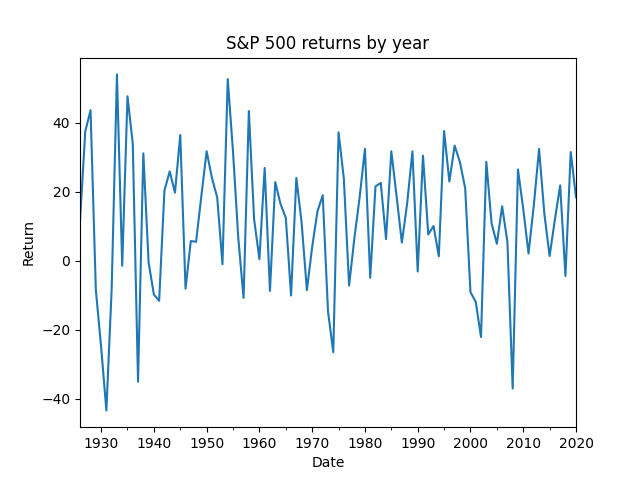
\includegraphics[width=.6\linewidth]{img/history.png}
    \caption{Stacionari laiko eilutė}
    \label{fig:sub1}
  \end{subfigure}%
  \begin{subfigure}{.5\textwidth}
    \centering
    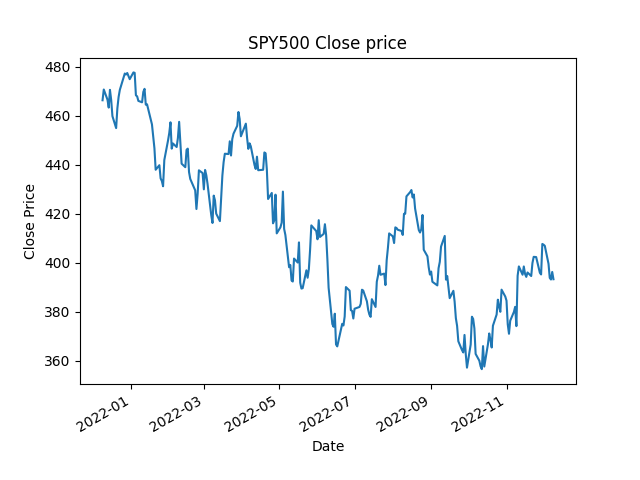
\includegraphics[width=.6\linewidth]{img/SPY_500_trend.png}
    \caption{Nestacionari}
    \label{fig:sub2}
  \end{subfigure}
  \caption{Stacionari ir nestacionari laiko eilutė}
  \label{fig:test}
\end{figure}

Grafai parodantys skirtumą tarp stacionarios ir nestacionarios laiko eilutės. Pirmajame (stacionariame) grafe yra pavaizduota vidutinis metinis pelnas
investuojant į SnP500 akciją nuo jos atsiradimo pradžios. Tai yra matoma ir vizualiai, jog imties vidurkis yra panašus visuose taškuose, taip pat
variacija ir kovariacija yra pasiskirščiusios panašiai visais laikais.
% sources!!!!!!!
% later after introducing AR models?
\subsection {ACF ir PACF}
ACF (angl. autocorrelation function) ir PACF (angl. partial autocorrelation function) naudojama analizuoti laiko eilutes. Pritaikant ACF bei PACF modelį 
galima lengviau parinkti ARMA, ARIMA modelio pradines reikšmes pagal atsilukusiuos kintamuosius.

% autoregression crypto currency predict
% ar, ar-abs, arima, arfima, sarima
\section{Autoregresiniai modeliai}
Vienas iš būdų analizuoti laiko eilutės yra autoregresija ir ją naudojantis modeliai. Egzistuoja ne vienas autoregresija naudojantis modelis. 
Populiarusi ir dažniausiai sutinkami modeliai yra ARMA(p, q) ir ARIMA(p, d, q).
Šie modeliai taip pat naudojasi anksčiau nepaminėtu MA modeliu kuris yra slankaus vidurkio modelis (angl. MA - moving average).
Taip pat yra SARIMA, SARFIMA ir kitų modelių, turinčių savo specifinius panaudjimo atvejus. 
Toliau apžvelgsime detaliau autoregresinius modelius ir kaip jie galėtų būti panaudoti iškeltiems užduotims šiame darbe spręsti.

\subsection{AR modelis}
AR (angl. autoregressive) modelis remiasi tik praeities duomenimis, kad nuspėti kintamojo reikšme ateityje, ieškoma ar pastebimas pasikartojantis
modelis, kuris padėtų tiksliau nuspėti dydį ateityje. Šis modelis dar dažnai vadinamas ARp modeliu, nes naudojamas kintamasis "p", nusakantis kiek praeiteis reikšmių 
iš laiko periodo norima naudoti. Laikant, kad kintamasis X yra laiko eilutės kintamasis AR(p) modelio formulė gali atrodyti taip: 
\[X_{t} = \Phi _{1}X_{t-1}+\epsilon_{t} \]

%\cite{chi2018stock} naudojami AR, MA ir ARMA modelio formulėms
${X_t}$ - stacionari laiko eilutė, $\Phi$ - AR modelio koeficientas, P - AR modelio laipsnis, $ \epsilon_{t} $ - AR modelio paklaida.

\subsection {MA modelis}
Toliau tyrinėjami autoregresyvieji modeliai susideda iš dar vienos dalies - Slankaus vidurkio - MA (angl. Moving average). Slenkančio vidurkio dabartinė
reikšmė tiesiškai priklauso nuo dabartines ir praeitų reikšmių. Žymėjimas MA(q) reiškia q laipsnio slenkamajį vidurkį, kurio formulę atrodo taip:  
\[X_{t} = \epsilon_{t} - \sum_{i=1}^{q}\theta_{i}  \epsilon_{t-i}\]

${X_t}$ - stacionari laiko eilutė, q - MA modelio laipsnis, ${\epsilon_t}$ - MA modelio paklaida.

\subsection {ARMA modelis}
% @article{makridakis1997arma}
ARMA (angl. autorogressive moving average) modelis yra autoregresyviaus ir slankaus vidurkio modelio junginys. Modelis dažnai žymimas
kaip ARMA(p, q), kur p yra AR laipsnis, o q yra MA laispnis. Pirmą kartą sujungtas 1938 mokslininko Herman Wold, jis pastebėjo jog ARMA modelis gal apimti 
dideles stacionarias laiko eilutes, kai yra tinkamai nurodytas p laipsnis ir q laipsnis. Taip pat reikia pabrėžti, jog ARMA(0, q) = MA(q) ir ARMA(p, 0) = AR(p)
Reiškia, jog Xt eilutė gali būti modeliuojama kaip kombinacija praeities $x_{t}$ reikšmių ir/arba praeities $e_{t}$ klaidų:
\[X_{t} = \phi_{1}x_{t-1} + \phi_{2}x_{t-2} + ... + \phi_{p}x_{t-p} + e_{t} - \theta_{1}e_{t-1} - \theta_{2}e_{t-2} - ... - \theta_{q}e_{t-q}\]


\subsection {ARIMA modelis}
ARIMA (angl. autoregressive integrated moving average) modelis yra paplitęs nuo 1970-ųjų iki šių dienų. Modelio pavadinimo šifravimas
pažodžiui: AR - Autoregresinis modelis, I - Integracija (Diferencijavimas), atsižvelgiama į duomenų tendenciją, MA - (Moving average) slankusis vidurkis.
AR ir MA yra atskiri modeliai, kurie gali būti naudojami paprastesnei laiko eilučiu analizei. Šio modelio privalumas, jog jis sujungia AR ir MA naudojimą kartu su
diferencijavimu, kuris suteikia galimybė giliau analizuoti laiko eilutes. Diferencijavimo dalis turimus duomenis padeda paversti į stacionarius, 
kurie yra reikalingi korektiškam modelio veikimui. Diferencijavimas vyksta baigtinį kartų skaičių, jog būtų pasiekta beveik-validi stacionari būseną. 
Kitais žodžiais ARIMA yra ekvivalentus ARMA modelis tiem patiems MA ir AR laipsniams \cite{hua2020bitcoin}. Taigi ARIMA modelis yra paremtas ARMA modeliu. 
Pagrindinis skirtumas tarp šių modelių yra tas, jog ARIMA konvertuoja nestacionarius duomenis į stacionarius prieš dirbant su jais. Modelio tipas yra 
klasifikuojamas kaip ARIMA(p,d,q), kur p - autoregresyvoji dalis, d - integravimo (diferencijavimo) dalis, q - slenkančio vidurkio dalis. Visos ARIMA modelio
reikšmės yra neneigiami sveikieji skaičiai \cite{mondal2014study}.

% Not sure about this
% dažniausiai negalima naudoti šiame kontekste
Dažniausiai yra 3 žingsniai naudoti ARIMA modelį:
1. Duomenų surinkimas ir verifikavimas - tikriname ar gauti duomenys yra stacionarūs ir ieškome sezoniškumo.
2. Diferencijavimas - vertimas laiko eilutę į stacionarią.
3. Prognozavimas naudojant ARIMA modelį - dažniausias taikomas ARIMA modelis yra ARIMA(1,1,0)

% atskirti trumpos atminties ir ilgos taminties modelius?
\subsection {ARFIMA modelis}
ARFIMA (angl. autoregressive fractionally integrated moving average) modelis yra ARIMA modelio išplėtimas.
Šis modelis apibendrina autoregresyvų integruotą slankiojo vidurkio (ARIMA) modelį su sveikaisiais integracijos laipsniais.
Parametrizavimas sujungia autoregresyvų slankiojo vidurkio (ARMA) modelį, kuris yra plačiai naudojamas trumpos atminties procesu, taip 
patampant ilgos atminties procesu. ARFIMA tinka analyzuoti toliau į priekį lyginant su ARIMA trumpos atminties procesu \cite{samimi2009long}.

% parašyti kas tokie tiksliai yra p ir q
Atliekamos trys procedūros prieš pradedant naudoti ARFIMA(g,d,q) modelį:
Testuojama laiko eilutės ilgos atminties savybės ir nustatoma trupmeninio diferencijavimo parametrą d.
Trupmeniškai diferencijuojama laiko eilutė, ko pasekoje gaunamas ARMA procesas.
Nustatomi kiti du ARFIMa modelio parametrai p ir q.
% šis modelis iš esmės 

\subsection {SARIMA modelis}
SARIMA (angl. seasonal autoregressive integrated moving average) modelis yra ARIMA modelio išplėtimas turintis vieną papildomą savybę - sezoniškumą. 
Pastebėjus, jog periodiškai kartojasi rezultatai laiko eilutėse, galima taikyti šį modelį. Geras ir paprastas pavyzdys, prekyba šventiniu laikotarpiu - kalėdos.
Prekybos centruose, tuo metu padidėja prekybą, tačiau kitą mėnesį ženkliai sumažėja. Spartus sumažėjimas nereiškia, jog prekybai yra didėlės problemos ir reikia pokyčių.
Tai dažniausiai yra žmonių poilsis nuo pirkinių po šventinio laikotarpio. šis modelis pastebi panašius sezoniškai atsitinkančius įvykius, juos atpažįsta ir pritaiko naudojant
ankščiau minėtą ARIMA modelį. 

\subsection {SARFIMA modelis}
SARFIMA (angl. autoregressive fractionally integrated moving average) modelis yra SARIMA modelio papildymas naudojant integravimą trupmenomis.

\subsection {AR-ABS}
%autoregressive - asset backed security

\section{Robotas lošėjas}
Taigi po literatūros analizės galima pradėti modeliuoti robotą.

\subsection{Roboto veiksmai?}
% Taigi valiutą perkame jeigu gauname signalą pirkti, kitu atveju robotas skanuoja duomenis nustatyta periodą. Pirkimui naudojamas "Moving Average" algoritmas. 
% Vartotojas pats gali nustatyti norimą intervala šiam algoritmui, tačiau rekomenduojamas intervalas yra kuo mažesnis, nes kriptovaliutų rinka 
% yra nepastovi ir greitai keičiasi 

% autoregression crypto currency predict
%\subsection(Auto regressive - ABS)

\section{Rezultatai}
Atlikta mokslinė analizė, literatūros apžvalga, kurios dėka pavyko aiškiau suprasti darbinę sritį ir pasigilinti į 
tyrinėjamą dalyką. 
Palyginti autoregresiniai modeliai ir kuo jie skiriasi, surastas tinkamiausias esamoje situacijoje modelis
Padėti pamatai kurti robotui, susipažinta kokią darbinę aplinką teks naudoti, python ir python-binance biblioteką.
Pritaikyti "Binance" testiniame tinkle parinkti autoregresniai modeliai ir gauti rezultatai

% Išvadose ir pasiūlymuose, nekartojant atskirų dalių apibendrinimų,
% suformuluojamos svarbiausios darbo išvados, rekomendacijos bei pasiūlymai.
\sectionnonum{Išvados}
Taigi matome, jog galima kurti robotą kuris prekiauja remiantis autoregresiniais modeliais.
\begin{itemize}
  \item Geriausi rezultatai gaunami naudojant ARIMA modelį (pavyzdys);
  \item Dar viena išvada;
  \item Paskutinė išvada;
\end{itemize}
Neišvengiama, jog tokiame trumpame darbe būtų aptartos visos įmanomos sritys ir atvejai, taigi tolimesnei tyrimo eigai pasiūlymas nagrinėti prognozuojamus modelius, 
kurie naudoja dirbtinį intelektą. Suprasti jų veikimą ir palyginti su standartiniais statistiniais prognozavimo būdais aptartais šiame darbe arba kitais nepaminėtais
prognozavimo modeliais (VAR, GARCH). Šiame darbe apsistojama ties kainų tendencijų prognozavimų, tolimesnė programos galima eiga būtų realizuoti pritaikyti konkrečias strategijas 
robotui lošėjui, kuris pagal gautas prognozes atlieka atitinkamą veiksmą.

\sectionnonum{Sąvokų apibrėžimai}
\textbf{Kriptovaliuta} - Kriptovaliuta yra skaitmeninė arba virtuali valiuta, kuri yra apsaugota kriptografija, todėl beveik neįmanoma jos padirbti ar išleisti dvigubai.

\textbf{Kriptovaliutų pora} - Kriptovaliutų pora rinkoje yra naudojama prekiaujant. Kriptovaliutos yra susietos poromis, tad norint nusipirkt BTC valiutos pirmiausia reikia surasti 
galimus keitimo variantus, jei egzistuoja pora BTC/BUSD, galima nusipirkti BTC kriptovaliutos uz turimas BUSD valiutas. Dažnu atveju rinkoje pasidėjus ("FIAT") valiuta
prekybos rinką ją konvertuoją i panašių token valiuta kaip BUSD(us -regulated stablecoin), USDT (usd tether) ar BNB (binance coin)

\textbf{API} - Aplikacijų programavimo sąsaja (angl. Application programming interface), tai sistemos suteikiama sąsaja, kuria galima naudotis norint pasiekti tos sistemos
funckionalumą ar apsikeisti duomenimis.

\textbf{Slankusis vidurkis} - Finansų srityje akcijos ar kito prekiaujamo objekto kainos vidurkio tam tikru periodu rodiklis. Vidurkio skaičiavimo priežastis - padėti išlyginti
kainos duomenis nuolat atnaujinant vidutinę kainą.

% TODO: autoregresinis ar autoregresyvus
\textbf{Autoregresinis modelis} - Statistinis modelis yra autoregresinis, jei jis numato būsimas reikšmes pagal praeities reikšmes. Pavyzdžiui, autoregresinis modelis gali
siekti numatyti būsimas akcijų kainas, remiantis ankstesniais rezultatais.

\printbibliography[heading=bibintoc] % Literatūros šaltiniai aprašomi
% bibliografija.bib faile. Šaltinių sąraše nurodoma panaudota literatūra,
% kitokie šaltiniai. Abėcėlės tvarka išdėstoma tik darbe panaudotų (cituotų,
% perfrazuotų ar bent paminėtų) mokslo leidinių, kitokių publikacijų
% bibliografiniai aprašai (šiuo punktu pasirūpina LaTeX). Aprašai pateikiami
% netransliteruoti.

\appendix  % Priedai
% Prieduose gali būti pateikiama pagalbinė, ypač darbo autoriaus savarankiškai
% parengta, medžiaga. Savarankiški priedai gali būti pateikiami kompiuterio
% diskelyje ar kompaktiniame diske. Priedai taip pat vadinami ir numeruojami.
% Tekstas su priedais siejamas nuorodomis (pvz.: \ref{img:mlp}).

% \section{Roboto veikimo struktūra}
% \begin{figure}[H]
%   \centering
%   \includegraphics[scale=0.5]{img/DIAGRAM}
%   \caption{Paveikslėlio pavyzdys}   % Antraštė įterpiama po paveikslėlio
%   \label{img:diagram}
% \end{figure}

\end{document}
